\chapter{Agent Design}
Developing a bot requires some forethought, even in agile development. The base of the bot must be both robust and versatile in order to accept future features. In this chapter the agents' gameplay strategy will be described as well as its architecture and implementation design.

Before any strategies for mid-game or late-game can be devised, the bot must first master early-game. If the bot loses in early-game, the match will never proceed to later stages. Compared to matches between humans, the game usually ends much quicker, rarely leaving early-game. This is because later stages of the game involves many more kinds of units and strategies, such that the AI must be more advanced. Therefore, it seems prudent to first perfect the early game of the bot. From there, if time allows, the bot could attempt mid-game tactics.

Simplest solution is implementing one strategy, which can be expanded into mid-game if the round drags on that long. Both boom and turtle strategies seek to push the match out of early game, so the remaining strategy which lies in early game is rush. This has seen a lot of use in the bot tournaments, probably being the most popular choice. It requires nothing but building the earliest combat unit and attacking. When moving on to mid-game, additions could include upgrading, expanding to new resources or moving on to more advanced units. Even a failed rush would put pressure on the opponent, allowing the bot to compete in later stages of the match. This makes such a strategy sustainable in case the bot reaches mid-game, but is also proven to be a strong early-game strategy.

Bots focus on a single race, as there is no advantage the capability to play more. In this case, this bot will play Protoss. Even though Protoss are the slowest of the three to produce the first troops, they have the strongest and easiest to use early troops. This makes it a strong rush candidate, as it can easily beat opposing races' rushes if prepared. While the main AI challenges between races are shared, gameplay elements differ quite a lot.

\section{Architecture Design}
The imperative when designing the bot is to lessen the decision space as greatly as possible. The problems the bot faces are easily divided into smaller, isolated problems. Its therefore possible to construct the bot out of individual \emph{modules}, each solving some subset of problems. This isolation lessens the amount of concurrent decisions and information available to the agent, reducing the decision space.

These modules are structured in a \emph{hierarchy}. A superior module can command a subordinate, however only in terms of a \emph{black box}, without knowledge of its internal structure. By limiting the information available to the superior, we can easily limit the decision space with clever design. The clear benefit of this structure is easy replacement of individual modules, without damaging or refactoring neighbors. On the other hand, modules will inherently be limited with information, but we must trust that not all available data is required or even relevant for all decisions.

The UAlberta bot by Dave Churchill uses such a module structure, however it places them in an interesting hierarchy. The modules in the bot are in a \emph{arborescence} graph structure, that is, there is a root module which has exactly one path to each other node in the hierarchy. In other words there are no cyclic dependencies, and it is related to a tree structure, except a single module can have multiple parents. Churchill alleges that it is based on "proven military structures" - in any case the UAlberta bot is high-ranking bot, victor of one competition and runner up in others. The data-structure must have been proven to work by now.

The benefits of this structure is lesser and easier dependencies, removing the inherent challenges in cyclic dependencies. It enhances the benefits of modular design, since modules has a stricter position in the hierarchy, making the modular design easier. It is also a great boon to agile development, as the tree will simply evolve upwards with newer modules as superiors to the older. The lower modules make smaller decisions with fewer resource such as building and gathering, and the higher modules control more information to make the larger scale decisions such as strategies and attacking.

On the other hand, the structure allows less complicated interactions. By limiting the hierarchy, the information available is limited as some modules must be at the bottom of the hierarchy. These are inevitably void of interactions with higher modules. This is also felt at the root of the structure, as at some point all the choices have to be made in the final module.

\begin{figure}
	\centering
	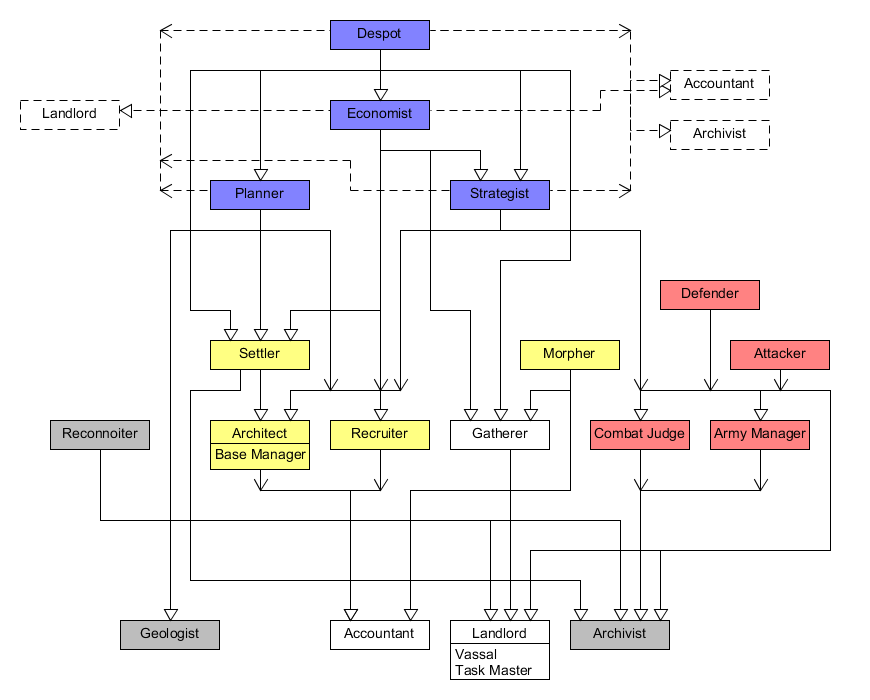
\includegraphics[width=\textwidth]{figures/Hierarchy}
\caption{Diagram of the module hierarchy.}
\label{fig:hierarchy}
\end{figure}

Figure \ref{fig:hierarchy} depicts the hierarchy structure, where higher modules are dependent on lower, shown by the arrows. The dependency is a one-way communication, such that the superior can query and operate its subordinates, but they are oblivious to their superiors. Modules which has direct subordinates only they are superior to are shown in the same box for simplicity.

The modules are separated in categories of interests, where likewise colored modules handle similar objectives. In the following chapters, we will explain the modules in the hierarchy and the underlying problems they solve.

\begin{itemize}
	\item Chapter \ref{ch:resources} (green) explains the concepts of resources and workers in StarCraft and how they are managed.
	\item Then, Chapter \ref{ch:production} (yellow) covers training and building units, which requires the resource modules.
	\item Information and its management is the subject of Chapter \ref{ch:exploration} (gray), which also covers scouting,
	\item which attacking, defending and general combat, detailed in Chapter \ref{ch:combat} (red), is dependent on.
	\item At the root of the hierarchy is economy and strategy, which is described in Chapter \ref{ch:strategy} (blue).
\end{itemize}

Finally, Chapter \ref{ch:results} presents and discusses the results of the bot and the project.

\section{Implementation Details}
\emph{BWAPI} is an API for StarCraft Broodwar and is injected upon startup by \emph{ChaosLauncher}. It loads an AI module written in C++, which can retrieve information about the current match's map status and send commands to the game through BWAPI. This controls the player's actions and allows the development of bots for StarCraft.

Depending on the settings in BWAPI, the agent can be disallowed to retrieve information a player would not be able to. This means some units are in some levels of accessibility, where invisible and destroyed units are completely inaccessible. This has some limits however, as the agent can retrieve information about burrowed and cloaked units as if they were not. While a keen player can spot these units as they are not completely transparent, the agent has no limits as if they were completely visible, giving it an advantage. Additionally the agent is not limited to what is visible currently on the display, but can retrieve information from all over the map.

There is a popular library, the \emph{Broodwar Terrain Analyzer} or \emph{BWTA} for short, which pre-processes maps for locations of interest. Most importantly, it marks the optimal depot locations for gathering resources. While BWAPI already does this for start-locations, BWTA also does this for all resource clusters, marking viable expansion locations. The pre-processing of the map only has to be done once as the results are stored for subsequent games on the map. This library is automatically included in the 3.7.4 BWAPI test bot, so it is probable that almost all bots use the library.

While newer versions of BWAPI exist, the 3.7.4 version is still widely used as it is considered the most stable, and is compatible with BWTA. There does exist a BWTA clone for 4th versions, however it is not very stable. The downside to 3.7.4 is that it does not support C++11, so C++98 had to be used. There does not exist an equivalent to BWAPI for StarCraft 2, since technically BWAPI is a hack and using it would result in a ban. AI's have been scripted in StarCraft 2's own editor however, and some have even gone and interpreted the display output of the game for a bot.

	\subsection*{Programming Details}
	Each module is its own class, where subordinates are given as arguments upon instancing. Beyond the root module of the hierarchy, there is the actual AI module called \emph{Primary}, which is the one loaded into StarCraft. It receives all the callbacks from BWAPI, delivering them to the appropriate modules. It is also responsible for creating the hierarchy upon construction and updates it each frame. Modules are updated from bottom to top, such that subordinate dependencies are current at all times.
	
	Almost everything a player is capable of interacting with through the game interface is handled as a simple method by BWAPI. Commanding units for example is simply calling the appropriate method on the unit-pointer. A more generic technique is used here however, where a unit, a target location and/or unit and a command type is given as arguments instead. This is to generalize the act of commanding, which requires a fair few checks such as whether the unit already has received a command this frame.
	
	A simple version of the hierarchy was designed initially in the project, but later iterations were done with no design beyond the current feature(s) worked on. Every module has been refactored multiple times as a result of the agile development, especially those lower in the hierarchy such as the Landlord.
	
	Some C++ STLs were used for their data-structures or writing to a stream. \emph{BOOST} libraries were used for their macro for-loops, capable of some C++11 functionalities lacking in C++98. Use of dynamic memory was avoided as much as possible because of the risks of memory-mismanagement. Only the \emph{Vassals} from Chapter \ref{ch:resources} use them.
	
	Every method has a brief comment describing its input, return and possible modifications to the object. Almost every scope beyond one line has a single line summarizing the current scope, since some methods can get quite large.